\subsection{新赛季规则解读}

    \subsubsection{整体规则分析}

    \subsubsection{比赛机制调整}

    \subsubsection{场地调整}

    \subsubsection{各兵种规则分析}

        \paragraph{步兵规则分析}

            \setlist[itemize]{label=\raisebox{-1.2ex}{\scalebox{3}{$\textbullet$}}}
    
            \begin{itemize}
                \item 25赛季可在准备3分钟内预装弹,且不再限制初始预装弹数量,根据以往比赛经验,要求步兵机器人至少拥有400发的预装弹量。本赛季现有设计中,步兵机器人预装弹量已满足要求,但机械组仍需尝试在不牺牲其它性能的前提下继续扩大预装弹量。
                \item 25赛季步兵通往关键交战区中央高地共有四条可选路径:翻越小资源岛台阶、公路区、公路隧道、高地隧道。由于普通步兵不具备翻越台阶的能力,故小资源岛台阶不予考虑;公路区与公路隧道需要经过颠簸路段,且公路区路程较长,考虑25赛季新增使用能量总额限制(20000焦),为减少功耗,普通步兵在非必要情况下应避免选择这两条路径;高地隧道路程短且无需经过颠簸路段,是普通步兵出入中央高地的最佳路径,因此本赛季普通步兵机器人必须具备穿越隧道的能力,这就要求机械组必须设计出尺寸合适,能够穿越隧道的机器人。此外,步兵可通过飞坡直达敌方公路区,从而阻击敌方英雄吊射以及快速接近敌方基地区,这要求本队步兵机器人机械组必须研发出重心适中,具备稳定飞坡能力的步兵机器人。
                \item 相较于24赛季,平衡步兵的概念以及经验加成等规则红利被取消,归类到普通步兵,从前后两块大装甲板变为了四块小装甲板,更容易被对方机器人打击,看似轮腿步兵相对于普通步兵毫无优势,但因为其功率计算的特殊性,使得它能够在一个较小的功率内仍有较快的移动速度,进攻、回防速度快,同时可以限制对方英雄吊射;并且五连杆机构给予了轮腿步兵很强的灵活性,能够轻松通过起伏路段,实现蹭台阶和飞坡等地形跨越动作来获得地形跨越增益,因此轮腿步兵在比赛中应该充当速攻、抢点、回防的角色。
                \item 25赛季堡垒增益点仅在己方前哨站被击毁,且基地血量落后时生效,可被一台哨兵或步兵占领,获取无敌、枪口热量、发弹量等增益,在防守基地区时拥有巨大优势。当基地区遭到入侵且哨兵不能优先占领堡垒点时,步兵应积极占领堡垒点。
                \item 25赛季能量机关可由任意机器人激活,但出于经济考虑,激活能量机关的最佳选项仍是机动性最高的步兵,此外,激活能量机关后会为基地和前哨站带来防御增益,为机器人带来攻击增益,使得队伍更容易展开进攻或进行防守,因此能量机关的激活将是本赛季的重中之重。
                \item 25赛季步兵机器人仅靠发射弹丸、或在 3 分钟内对前哨站造成 500 点伤害、或成功击打对方机器人所带来的经验值是不足以升级的,这要求步兵机器人在本赛季要做到快速精准的打击,并与队友制定相关战术策略以更快提升等级。进攻时,步兵机器人应积极占领中央高地区域,为己方英雄和步兵带来增益,对对方机器人造成更有力的打击,防守时积极占领堡垒、前哨站和基地区,获取防御增益进行反击。
                \item 对于轮腿步兵,除上述占领增益点外,还能在飞坡点和公路区地形跨越增益点进行交互获得增益,因此要求电控的算法要具备很强的稳定性。
                \item 操作方面,25赛季与24赛季一致,可选择手动控制或半自动控制。半自动控制相比24赛季,增加了25\%的防御增益。半自动步兵在数值上将会比手动控制步兵有更大的优势。	
                \item 25赛季新增底盘能量总额20000焦限制,一旦超出限制,则机器人的功率永久削减,因此,本赛季应制定能量使用策略,减少非必要的能量消耗。
            \end{itemize}
        
        \paragraph{步兵策略战术}
    
            \setlist[itemize]{label=\raisebox{-1.2ex}{\scalebox{3}{$\textbullet$}}}
    
            \begin{itemize}
                \item 步兵在具有高机动性和灵活性的同时,对前哨站和基地的伤害收益小,且血量较少,因此步兵在比赛中的主要职能为占领增益点、掩护和支援我方其它机器人单位、阻击敌方英雄、攻击敌方地面机器人以及协同激活能量机关。
                \item 在开局针对中央高地的争夺战中,轮腿步兵因为功率计算和五连杆机构的特殊性,具有较强的机动性,可以通过蹭台阶迅速占领中央高地增益点并对对方机器人进行打击,同时,我方步兵应当尽量避免进入敌方哨兵的索敌范围。
                \item 当己方英雄吊射命中率较高时,步兵优先选择掩护英雄,防御敌方飞坡步兵;当英雄吊射命中率偏低时,选择从香蕉道到对方区域干扰敌方英雄吊射(具体能否实现需要看最终的尺寸),以及攻击敌方地面机器人。
            \end{itemize}
    
            \begin{figure}[H]
                \centering
                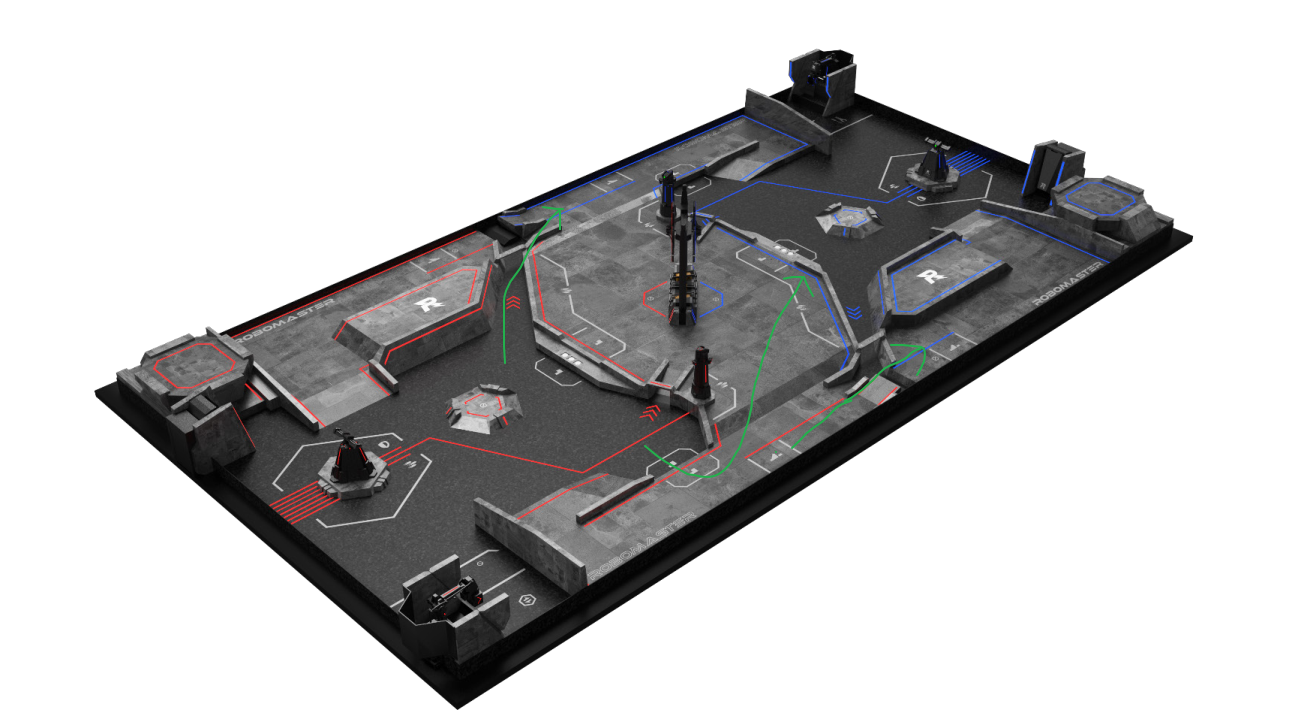
\includegraphics[height=0.35\textwidth]{figure/infantry_tactics.png}
                \hspace{0.5em}
                \label{fig:infantry_tactics}
            \end{figure}

        \paragraph{英雄规则分析}

            \setlist[itemize]{label=\raisebox{-1.2ex}{\scalebox{3}{$\textbullet$}}}
    
            \begin{itemize}
                \item 今年的英雄机器人引入了“部署模式”,在己方半场内,英雄机器人可通过2秒的确认时间进入“部署模式”,底盘断电后获得25\%的防御增益,并获得狙击攻击增益与经济加成。这一机制的引入,英雄在己方半场的任意位置,对敌方基地造成可观的伤害输出。“部署模式”需要其他兵种的协同支持,为团队协作和战术规划提供了更多可能性。同时规则对适用于部署模式的“比赛节奏”做出了一些限制,开局有2次命中能享受部署模式加成,此后每20s增加一次机会。
                
                \item 今年新增的42°坡提升了地形复杂度,对英雄机器人的底盘设计和功率分配提出了全新要求。传统的麦克纳姆轮加上英雄机器人的重量难以胜任这一高难度场景,地形上鼓励其他底盘结构(例如舵轮底盘)。42°坡本身是一个极具战略价值的狙击点,占领这里可以对战局产生重要影响。同时这一位置容易受到对方无人机的威胁,对时机的精准把控至关重要。解决这些技术难点,我们就能在比赛中抢占先机,充分释放英雄机器人的潜能。
                
                \item 能量体系:今年的规则更新中,英雄、步兵、哨兵机器人在底盘能量消耗达到20000J后将进入“虚弱”状态,对于比赛节奏和战术规划有新的要求。这一规则也对电容的性能和整车的能量控制系统提出了更高要求。如何提升电容效率、优化整车能量管理,将成为提高胜率的关键技术突破点。
                
                \item 赛制时间分析:在新赛季中,空中支援机制进行了调整,英雄在前30秒需要占领梯形高地、准备击打前哨站,30秒后将与无人机和对方英雄机器人形成制约。地形变化使得梯形高地的防御增益对英雄机器人的吊射和部署模式至关重要。若某方的梯形高地增益点仅被该方机器人占领,则在比赛的不同时间段(2-3分钟、3-5分钟、5-7分钟),占领的机器人可获得2、3、5倍的枪口热量冷却增益和25\%的防御增益。
                
                \item 雷达机制分析:雷达可以向所有己方机器人发送数据,接收哨兵机器人的数据。新规则下英雄吊射点位更加灵活,但在部署模式下底盘处于“失能状态”,此时很容易陷入被动。对于吊射点位的选择,可以通过感知敌方位置,为英雄操作手实时更新可以进行吊射的位置;或直接检测预设的吊射点位是否有敌方单位,方便操作手进行决策,提前预警,减少被抓风险,提高灵活性。还能在敌方进入基地范围内时,向英雄操作手发送”防守”的决策信号,调动英雄回防。
    
                \item 英雄狙击模式下,命中敌方基地会获得50金币。英雄狙击伤害可获得100经验值,跟上赛季一样,但是区别在于这赛季英雄新增的部署模式,可以随时狙击。也就是说英雄如果能利用好这个狙击能大大增长升级速度,同时前期也可以使用狙击击打较好命中的目标,加速升级。
    
                \begin{figure}[H]
                    \centering
                    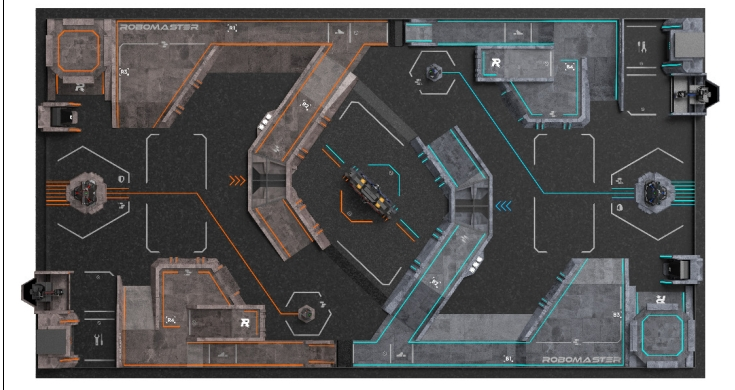
\includegraphics[height=0.35\textwidth]{figure/RM2024_map.png}
                    \hspace{0.5em}
                    % 添加居中、黑体、加大的字体
                    \caption{\textbf{\zihao{-4}\textbf{RM2024场地示意图}}}
                    \label{fig:RM2024_map}
                \end{figure}
                
                \begin{figure}[H]
                    \centering
                    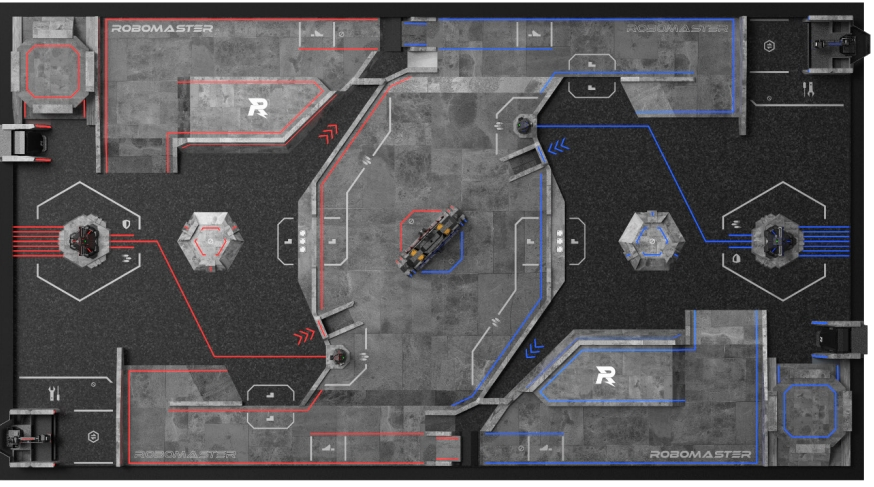
\includegraphics[height=0.35\textwidth]{figure/RM2025_map.png}
                    \hspace{0.5em}
                    \caption{\textbf{\zihao{-4}\textbf{RM2025场地示意图}}}
                    \label{fig:RM2025_map}
                \end{figure}
    
                \item 场地中央的环形高地更换为中央高地,进入中央高地的路径也完全更改——24赛季可以由基地区直冲环形高地,但25赛季将公路区和中央高地直接连接,阻断了基地区直冲中央高地的行为,影响了英雄机器人冲锋的效率。并且中央高地和梯形高地改动,导致飞坡后英雄的路线选择减少,加大了飞坡的风险,由此可能要重新考虑飞坡的进攻价值性。
    
                \item 而中央高地的20°坡、狗洞和弯曲的香蕉道狭道,对于目前战队的英雄机器人而言是无法通过的,战略意义不大。如果后续场地不加以大的改动,可以尝试制造一台超小英雄过此类狭窄通道。
    
                \begin{figure}[H]
                    \centering
                    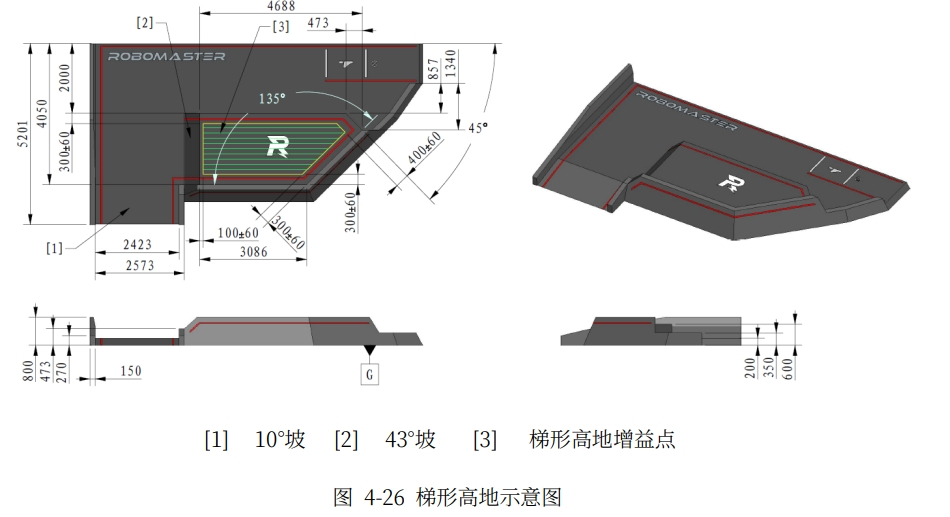
\includegraphics[height=0.35\textwidth]{figure/trapezoidalElevation.png}
                    \hspace{0.5em}
                    \caption{\textbf{\zihao{-4}\textbf{梯形高地场地示意图}}}
                    \label{fig:trapezoidalElevation}
                \end{figure}
    
                \item 梯形高地最受瞩目的就是43°高地,600cm的高度让能够上到这个高地的英雄机器人安全性得到了保障,目前看来所有兵种之中对在高地上有较大威胁的是平衡步兵和无人机。此高地还是全场中最适合吊射基地的位置,且距离前哨站只有7~8米的距离,还没有任何的障碍物遮挡视野。可以说,它就是提供给英雄的专属发射场地,重要性不言而喻,所以己方梯形高地是英雄前期必须尝试占领的战略要地。在前哨站失守的中期焦灼阶段和后期进攻阶段都可以尝试飞坡占领敌方梯形高地,为英雄自己创造一个较为安全的输出基地环境。但实现上坡对于英雄机器人的性能有一定要求,不管是轮毂影响,还是整个底盘通过角和重心位置设计,对于每一个队伍都是一个大的挑战。
                
                \begin{figure}[H]
                    \centering
                    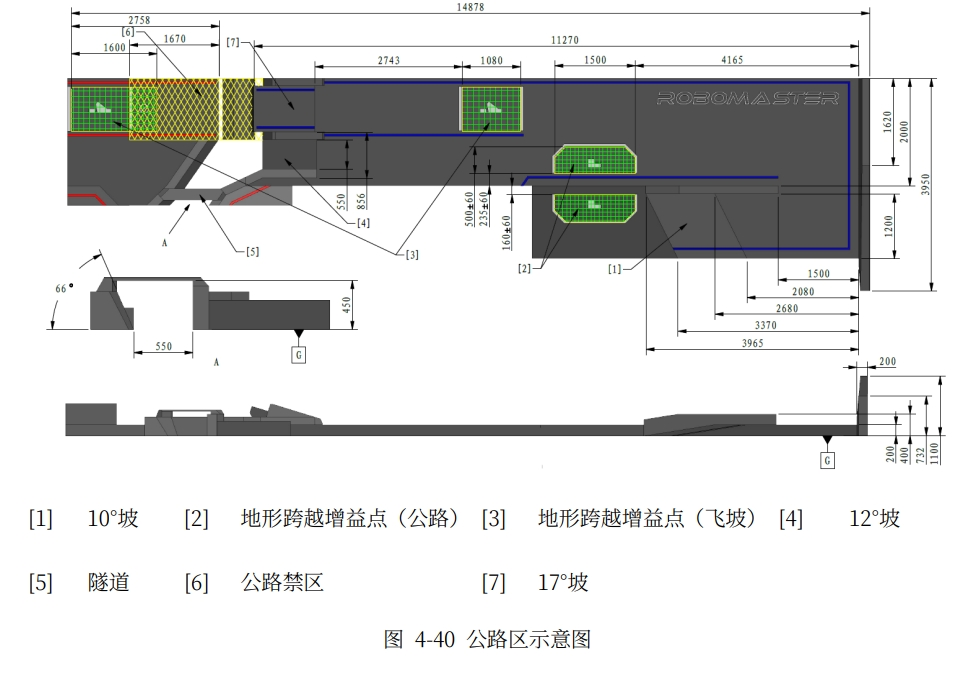
\includegraphics[height=0.35\textwidth]{figure/highwayArea.png}
                    \hspace{0.5em}
                    \caption{\textbf{\zihao{-4}\textbf{公路区场地示意图}}}
                    \label{fig:highwayArea}
                \end{figure}
    
                \item 直角弯对英雄机器人的转弯性能提出较高的水平要求,虽然在机械结构上麦轮底盘和舵轮底盘是可以通过,但对于操作手来说需要有熟练的操作才能减少过弯时间,避免磕碰,提高进攻效率。飞坡区域直接衔接到敌方梯形高地,并且只有梯形高地一条路可以走,一旦被敌方察觉并派遣机器人堵在梯形高地的出口,那么飞坡过去的英雄只能被瓮中之鳖,除非明确知道敌方所有机器人分布位置。在战略规划上,若非紧急情况不推荐英雄飞坡,但在功能规划上,英雄要具备飞坡功能。在通过与中央高地衔接部分和香蕉道的上坡部分,英雄机器人需要注意的是在进攻时段是否有敌方的步兵机器人存在,进攻或撤退时需要保证自身安全,此外没有任何其他过多要求。
    
    
                \begin{figure}[H]
                    \centering
                    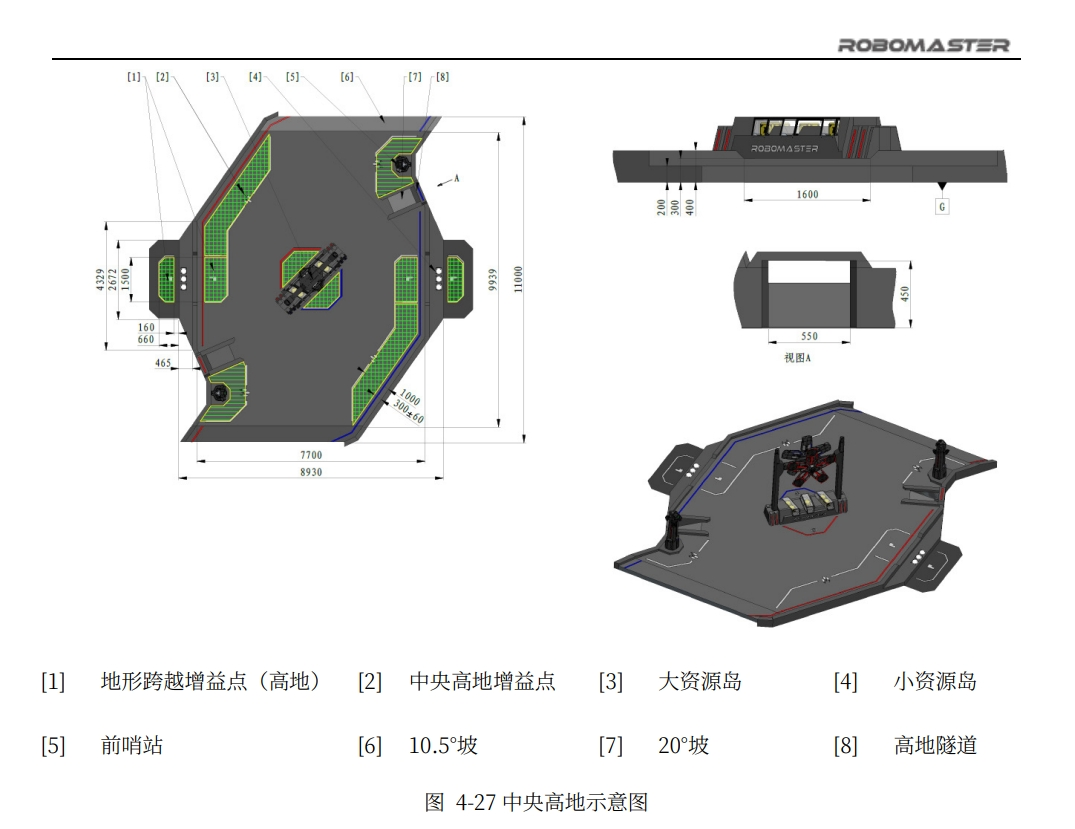
\includegraphics[height=0.35\textwidth]{figure/centralTableland.png}
                    \hspace{0.5em}
                    \caption{\textbf{\zihao{-4}\textbf{中央高地场地示意图}}}
                    \label{fig:centralTableland}
                \end{figure}
    
                \item 关于中央高地英雄机器人需要注意的就是颠簸路段、敌方“香蕉道”入口、狗洞以及敌方公路区出口。对机器人在性能有较高要求的就颠簸路段,在机器人制作中需尽量减少颠簸的影响性,但在多年比赛的经验来看,过颠簸路段时,无法发射,无法防御,只能快速通过,不然只能当活靶子。当英雄机器人在中央高地的时候,一定要时刻注意背后的香蕉道入口,中央高地四通八达,前后都有可能面临来敌。
    
            \end{itemize}

        \paragraph{英雄策略战术}

            \setlist[itemize]{label=\raisebox{-1.2ex}{\scalebox{3}{$\textbullet$}}}
    
            \begin{itemize}
                \item 出门左拐就是梯形高地了,英雄在比赛开始后可以尝试站住,攻击敌方前哨站,并为己方提供对于中央高地的态势感知。在设想中,梯形高地的落差同时也可为英雄提供对低处攻击的掩蔽,因此这里应该是英雄经常来的地方。
                \item 部署机制以底盘断电为代价换取一系列加成,虽然此时英雄有25\%防御增益,但在潜在的陆空威胁下仍十分脆弱。在地形复杂且四通八达的环境下,要求己方为英雄构建安全的“堡垒地带”显然难度较高,为此英雄操作手应该留意敌方无人机与地面机器人的出动与补给节奏(后半场可能的充电高峰期),见缝插针地抵近输出敌方前哨站与基地,并在危险来临时及时转入防守。
                \item 虽然组委会提过会增加飞坡之后的可选路径,但目前跨过沟壑之后,撤退的路径会经过敌方堡垒区,极有可能一去不复还,从敌方的角度而言飞坡的风险增大了不少。但同时加高的梯形高地也为到达敌方半场的机器人提供了更好的掩体。如果是快结束了想放手一搏可以考虑考虑。
                \item 无论是爬坡上梯形高地还是绕道己方公路区前往中央高地都势必会消耗不少能量,因此英雄应精打细算,增大补给间隔,并在比赛进行到下半场时择机在补给区“充电”。
                \item 对于底盘能量20000J的分配,前期应集中在占领梯形高地,中期寻找不同的部署点攻击对方基地,后期则需退回基地区拦截敌方步兵和英雄.
            \end{itemize}

        \paragraph{哨兵规则分析}

            \setlist[itemize]{label=\raisebox{-1.2ex}{\scalebox{3}{$\textbullet$}}}
    
            \begin{itemize}
                \item 哨兵在这个赛季的机制改动相当大,主要的改动在于哨兵取消了与前哨站挂钩的无敌机制、哨兵与比赛胜负的判定机制以及哨兵巡逻区的取消。此外,哨兵的初始发弹量也从400发削减到了300发,而且虽然底盘功率上限未做改动,但是哨兵和步兵、英雄一样适用于全局20000J底盘总能量的约束。这些改动无疑削弱了哨兵的单兵作战能力,也进一步提高了哨兵对完善的导航避障、自身定位、全局规划、灵活决策、资源调度和与其他机器人打配合的需求。
                \item 哨兵在这个赛季的战场上也依旧存在着不小的优势:首先,这个赛季并未对哨兵的枪口热量上限、每秒冷却做改动,这保证了哨兵在可发弹量充足的情况下输出能力依旧恐怖,而且,每一分钟哨兵都可以通过导航到补给区补血补弹或者远程兑弹的方式补充发弹量,这些机制平衡了哨兵初始发弹量削减的影响,在导航完善和工程获取经济能力强的情况下哨兵的发弹量甚至可能只取决于预装的弹丸有多少;其次,哨兵虽然取消了与前哨站挂钩的无敌状态,但是初始数据400血量100功率上限(步兵满级数据)保证了哨兵前期的性能和生存能力在线,配合恐怖的火力,在前期哨兵在面对对面的地面输出单位是具有绝对的压制力的,而且哨兵可以远程兑换血量以及它的复活机制并未改变,这意味着原本弹尽粮绝、性命垂危的哨兵可能突然以一个较好的状态重返赛场,对敌方形成巨大的威胁;况且,这个赛季新增了哨兵可以占领的堡垒增益点,当堡垒增益点开启,哨兵占领之后依旧可以获得无敌、额外发弹量和额外的枪口冷却增益,这一改动大大增强了哨兵的防守能力。
                \item 这个赛季的机制变动使哨兵更加全能,不论是在进攻端还是在防守端都有着独特的优势。显然,本赛季的改动无疑是令哨兵机器人的技术栈更加接近于全自动机器人的本质。没有一个完善的决策体系的话,在全局资源的规划和调动上会出现不可忽视的问题;巡逻区的取消无疑是对哨兵如何及时的规划进攻和回防路线将会是导航和定位上的挑战。
            \end{itemize}

        \paragraph{哨兵策略战术}

            \setlist[itemize]{label=\raisebox{-1.2ex}{\scalebox{3}{$\textbullet$}}}
        
                \begin{itemize}
                    \item 哨兵的前期作战能力是所有地面机器人中最强的,在前期利用高性能迅速占领中央高地上的增益点的战术价值很高,不论是前压前哨站还是阻击对面攻势都会令对手很头疼。
                    \item 哨兵可以在能量机关激活的时候击打能量机关获得额外增益。
                    \item 哨兵能远程补弹,可以在自身增益足够高或敌方状态差时乘胜追击,或是在被动防御时 尝试突围、扭转局势。
                    \item 哨兵可以通过雷达通讯接口得到鸟瞰全局的数据,通过自主决策可以选择进攻、防守、配合其他机器人或者规避围剿。
                    \item 哨兵可以占据中央高地,对靠近高地的机器人进行阻击和对取矿的工程机器人进行拦截。
                    \item 哨兵能接收云台手发送指令,在必要的时候可以解决一些意料之外、情况紧急的情况。
                \end{itemize}

        \paragraph{工程规则分析}

            \setlist[itemize]{label=\raisebox{-1.2ex}{\scalebox{3}{$\textbullet$}}}
    
            \begin{itemize}
                \item 小资源岛变更:小资源岛依旧紧贴中央高地护栏外侧,但银矿由原来的半嵌入式改变为完全嵌入,从原来可以通过夹爪直接取出改变成要求工程机器人从上面将其拔出,对工程机器人的机构要求更加灵活。
                \item 前往资源岛的路径变更:原来前往大资源岛的路径可以通过前哨站然后直接登上大资源岛或者直接钻隧道,而25赛季登上大资源岛的路径更加灵活,在基地正方向新增一个高300mm的二级台阶,第一级是高为200mm的小资源岛,所以工程机器人可以设计一个灵活的机构来完成登岛直接抵达大资源岛,而且现在是公路区连接着中央高地,所以工程机器人也可以选择绕远路先通过公路区再上岛,而上公路区又有选择,可以通过上200mm高的台阶进入公路区,也可以通过爬10°坡上公路区进而前往大资源岛,所以工程机器人的构型可以有更多选择特别是在底盘上。
                \item 经济体制改变:删除了五级难度的兑矿等级,等比例增加了剩余难度等q级的金币数量,且比例提高了随着兑矿次数增多时最低可选择兑矿难度的金币倍率,且新增选择四级难度时,工程机器人需要在15秒的时间限制内,连续兑换2块矿石,若在时限内兑换成功,2块矿石的所得金币将依次连续结算,否则将不会获得任何金币的机制,这需要工程机器人需要有非常灵活的兑矿机构,且操作手需要对操作更加熟练。 
            \end{itemize}

        \paragraph{工程策略战术}

            \setlist[itemize]{label=\raisebox{-1.2ex}{\scalebox{3}{$\textbullet$}}}
    
            \begin{itemize}
                \item 工程机器人定位:根据 25赛季规则的改动,我们认为工程机器人在25赛季的定位更加 偏向于通过取矿-兑矿换取金币达到为团队提供经济的一个角色,为其他车组提供更好的 配置条件,为多样化的战术选择提供经济支持。
                \item 取矿机构:六轴机械臂+吸盘。考虑到维修成本和迭代的选择上,使用板材替代上届的机加工方案。同时考虑到6r型机械臂Link1和Link2电机的承重,决定在这两个关节中引入弹簧的重力补偿,去避免电机的发热,延长使用寿命。
                \item 底盘选择:月球车底盘。由于场地的变更,工程机器人可以选择跨台阶的方式直接登上大资源岛,为了更快的争夺金矿来提高团队经济,我们选择可以适应复杂地形的月球车底盘来实现跨台阶的目标,在轮组的选择上我们将采用麦克纳姆轮来实现底盘的转向。 抬升兼存矿机构:剪式抬升架+一键2/3银矿.
                \item 抬升架的选择:剪式抬升。由于六轴机械臂的操控,我们采用剪式抬升架来抬升,并且在上面安装取银矿机构,使得可以取2/3个矿,由规则手册中场地部分可知,每两个银矿的中心距离为270mm,一键3矿则需要540mm,是可以尝试并且完成的(就怕后面又改规则),同时银矿一开始距离地面200mm,完全抽出来则需要400mm,所以会做一个180度的翻转使其更加稳定并且为后期存矿做足准备。
                \item 自定义控制器:带有六个角传感器的大臂缩小机械臂,采用大臂构型缩小的自定义控制器,有利用操作手更加直观的操作机械臂的运动,并同时减少解算需求,并考虑在自定义控制器中融入移动、吸取等快捷功能,以提升工程在存取矿的能力。
                \item 上位机实现:上位机采用ros2和movelt,将实时获取大臂的六个角度并跟踪机械臂的构型,在需要存取矿时,上位机将实现一次性取矿的路径规划。
                \item 下位机:优化各部分通讯,尝试在下位机实现机械臂正逆解算。
            \end{itemize}

        \paragraph{飞镖系统规则分析}

            \setlist[itemize]{label=\raisebox{-1.2ex}{\scalebox{3}{$\textbullet$}}}
    
            \begin{itemize}
                \item 飞镖命中收益改变:25赛季飞镖命中的基地固定目标和随机固定目标的收益下降。具体表现为命中基地固定目标、随机固定目标为步兵和英雄机器人下降到200和600、随机固定目标命中扣除地方机器人血量由25\%改为10\%、命中固定目标由1000下调至625,命中随机固定目标由1200下调至2500。25赛季新增的随机移动目标,命中难度更大,但收益比24赛季的随机固定目标更高。随机移动目标命中提供2500点巨额经验,同时对方操作收界面遮挡15秒,且对方全部存活的地面机器人立即受到相当于各自当前上限血量25\%的攻击伤害、对方基地护甲立即展开。随机固定目标和随机移动目标的收益下降、随机移动目标收益巨大,使我们这赛季击打的目标确定在随机固定目标甚至随机移动目标上。
                \item 场地变化:对比24赛季,飞镖发射站的结构有所变化,三分钟准备阶段内,飞镖发射站闸门将保持闭合状态,飞镖系统需从飞镖发射站的后方放入。这意味着在准备阶段无法进行人工标定及预瞄,飞镖系统需要更有效的利用开启闸门后的时间,对飞镖系统纯视觉瞄准的速度以及精度都有一定的要求。25赛季飞镖发射站闸门的开启次数和时间节点从原本的开始比赛30秒后两次开启机会,变为了开始比赛30秒后一次和4分钟后一次且未使用的机会可以累加。这一改动使得前期无法集中使用飞镖,对于需要在前期使用飞镖获得更大战果的情况,飞镖的准度和命中的稳定性显得更为重要。对比24赛季,从场地尺寸上来看前哨站与飞镖发射站的相对位置变化较为明显,夹角从24赛季的6.6°变为了2.1°。除此之外,飞镖发射站和基地沿与战场长边平行方向的距离减少了640mm。
            \end{itemize}

        \paragraph{飞镖系统策略战术}

            \setlist[itemize]{label=\raisebox{-1.2ex}{\scalebox{3}{$\textbullet$}}}
    
            \begin{itemize}
                \item 飞镖定位:根据25赛季规则的改动,飞镖在25赛季的定位偏向于战略进攻单位,优势时与地面配合进攻,在局势焦灼时通过飞镖致盲效果实现局势逆转。
                \item 准备阶段:发射台是从后方开放放入飞镖系统,在赛前准备时间3分钟内不能人工标定前哨站与基地,因此决定在裁判系统自检的五秒内通过飞镖架的摄像头识别引导灯,标定前哨站并记录敌方基地方位。提前锁定目标方向。缩短飞镖发射时间。
                \item 目标选择:在基地随机移动靶和随机固定靶带来的巨大收益,本赛季飞镖击打的目标需往随机移动靶和随机固定靶靠拢,由此需要研发制导镖架和制导镖体的预研发。
                \item 发射结构:由于摩擦轮发射的飞镖发射架具有较多的不稳定因素,本赛季决定采用拉簧弹射的方式,解决了摩擦轮旋转转速不一致可能导致飞镖不在预估轨道上的问题,同时,拉簧可以为镖体提供稳定的发射能量。
                \item 战术选择:飞镖系统“致盲”的时间改动,增加了首次命中的的“致盲”效果的时间,这提高飞镖的命中的重要性,充分利用飞镖的致盲效果,配合地面单位对敌方发起进攻,对敌方进行火力压制,消灭敌方地面单位,为己方建立优势。
            \end{itemize}

        \paragraph{雷达系统规则分析}

            \setlist[itemize]{label=\raisebox{-1.2ex}{\scalebox{3}{$\textbullet$}}}
        
            \begin{itemize}
                \item 雷达可以为队伍提供敌方机器人的位置信息,提供视野给到队伍。
                \item 雷达可以通过裁判系统将位置信息发给己方单位,并且只能接收哨兵的信息
                \item 己方的雷达可识别对方地面机器人的位置,并将该机器人的坐标发送至裁判系统,若精度符合条件则能持续积攒标记进度,当标记进度大于等于100时被标记的对象回获得一个-15\%的防御增益。
                \item 当雷达每累计使对方机器人易伤 1 分钟(同时有多台机器人易伤时,时间不累加),将会获得 1 次触发“双倍易伤”的机会,雷达可以通过裁判系统主动发送命令消耗机会,并使当前所有正处于易伤状态的负防御增益数值由-15\%变为-30\%,持续 30 秒。每局比赛中,雷达至多可以触发 2 次“双倍易伤”。
            \end{itemize}

        \paragraph{雷达系统策略战术}

            \setlist[itemize]{label=\raisebox{-1.2ex}{\scalebox{3}{$\textbullet$}}}
        
            \begin{itemize}
                \item 精准识别出敌方机器人的位置信息,累计标记进度并发送信息给予队伍,为队伍增加优势。
                \item 当有双倍易伤的机会时,配合队伍需求,触发该效果。
                \item 识别出敌方机器人在某些特殊位置(如我方基地前、飞坡等)时,可以通过裁判系统向己方单位发送预警信息。
                \item 通过裁判系统接收哨兵传来的重定位的信息,更加精确的锁定部分目标。
                \item 协助英雄对地方基地进行吊射。
            \end{itemize}

        \paragraph{空中机器人规则分析}

            \setlist[itemize]{label=\raisebox{-1.2ex}{\scalebox{3}{$\textbullet$}}}
        
            \begin{itemize}
                \item 空中机器人相较于上个赛季改动最大的是再比赛开始即可起飞,起飞后可以通过花钱的方式续费,这无疑是对空中机器人的大增强,首先就是对于哨兵和英雄存在极其强大的压制力,并且对于大部分队伍也能开局清除前哨站。
                \item 空中机器人的限重减少,这一改动直接影响了空中机器人的设计,并且取消了中途补弹,如果想发挥空中机器人的最大优势,首先便是需要将空中机器人的整体做轻,并且是弹舱的设计要能容纳的下最少1500发弹,对于很多队伍来说相当于只能重新设计一台无人机。
            \end{itemize}

        \paragraph{空中机器人策略战术}

            \setlist[itemize]{label=\raisebox{-1.2ex}{\scalebox{3}{$\textbullet$}}}
    
            \begin{itemize}
                \item 前期刚开局,压制英雄前期的吊射,英雄的改动使得其可以随处吊射,对于前哨站来说也是非常有威胁,如果不针对英雄便会与上赛季一样,英雄轻易吊射,并且新增的43°高坡使得步兵更难第一时间针对对方英雄,因此空中机器人前期可以采取压制哨兵与英雄的打法,如果对方并没有很强势的英雄与哨兵则可以优先打击前哨站。
                \item 在中期时,空中机器人主要起到帮助己推进或是防守的角色,在对方英雄,步兵处于优势位置时,可以优先针对,并且对于信息的获取也是一大关键,空中机器人也能开能量机关为团队进一步提供帮助。
                \item 后期可能会遇见两方的功率消耗殆尽,或者难以攻入对方,亦或者是基地/前哨/哨兵,血量接近此时无人机如果还能有电量留存则可以起飞去消磨对方的血量,拿下关键点。
            \end{itemize}